\documentclass[a4paper, 12pt]{article}

\usepackage{cmap} % поиск в PDF lusepackage[2A]{fontenc} % кодировка

\usepackage[utf8]{inputenc} % кодировка исходного текста
\usepackage[english,russian]{babel} % локализация и переносы
\usepackage{amsmath, amsfonts, amssymb, amsthm,mathtools, float}
\usepackage{ stmaryrd }

% Рисунки
\usepackage{graphicx}
\usepackage{wrapfig}

\usepackage[left=2cm,right=2cm, top=2cm,bottom=2cm,bindingoffset=0cm]{geometry}

\usepackage{longtable}
\graphicspath{pictures}

\author{Балдин Виктор Б01-303}
\title{Работа 1.1.4 \\ Измерение интенсивности радиационного фона}

\begin{document}

	\maketitle
	\section{Аннотация}
	\textbf{Цель работы:} применение методов обработки экспериментальных данных
	для изучения статистических закономерностей
	при измерении интенсивности радиационного фона.
	\bigskip\\
	\textbf{Оборудование:} счетчик Гейгера-Мюллера (CTC-6), блок питания, компьютер
	с интерфейсом связи со счетчиком.

	\section{Теоретические сведения}
	В данной работе измеряется число частиц, проходящих через счетчик за 10 секунд, с помощью которого мы можем найти и количество за 40 секунд. Такие времена выбраны для того, чтобы продемонстрировать то, что при большем времени лучше выполняется нормальное распределение измеряемых величин и гистограмма более симметрична, чем при малых временах, когда при оработке лучше воспользоваться законом Пуассона.

	Если случайные события, такие как регистрация частицы счётчиком, однородны во времени и являются независимыми, то результаты их измерений подчиняются распределению Пуассона. Теория вероятности гласит, что в таком случае среднеквадратичная ошибка числа отсчётов, измеренного за некоторый интервал времени, равна квадратному корню из среднего числа отсчётов за тот же интервал:

	\begin{equation}
		\sigma = \sqrt{n_0}
	\end{equation}


	При проведении многочисленных опытов за $n_0$ принимается среднее арифметическое всех результатов
	$\overline n$, а стандартная отклонение $\overline n$ от $n_0$ может быть
	вычислена по формуле:
	\[ \sigma_{\overline n} = \frac{1}{N} \sqrt{\sum_{i=1}^N(n_i - \overline n)^2}, \] где $N$ - количество измерений, $n_i$ - результат $i$-того измерения. Относительная же погрешность составит: \[ \varepsilon_{\overline n} = \frac{1}{\sqrt{\overline n N}}. \]

	Рассмотрим счетчик, регистрирующий частицы. Найдем вероятность того,
	что при плостности излучения $\nu$ счетчик сработает $n$
	раз за время измерения. Для простоты будем считать, что
	счетчик обладает единичной площадью.

	Представим себе большое число совершенно одинаковых одновременно
	работающих счетчиков. Обозначим полное число счетчиков буквой $N$.
	Через них в секунду в среднем проходит $N\nu$ частиц, а за
	$dt$ пройдет $N\nu dt$ частиц. Если $dt$ достаточно мало, то за это время
	ни через один счетчик не пройдет двух частиц. Число счетчиков, через
	которые прошла частица равно $N\nu dt$, а их доля по отношению к общему числу
	счетчиков: $N\nu dt/N = \nu dt$. Вероятность того, что за время $dt$ через
	счетчик пройдет частица, равна $\nu dt$.

	Вычислим теперь вероятность $P_0(t)$ того, что за время $t$ через счетсик не пройдет ни одной частицы. Количество таких счетчиков в момент $t$ составляет $NP_0 (t)$, а в момент времени $t+dt$ равно $NP_0 (t+dt)$. Это число меньше, чем $NP_0 (t)$, потому что за время $dt$ их сисло убавится на $NP_0 (t)\nu dt$. Поэтому: \[NP_0 (t+dt) = NP_0(t) - NP_0 (t)\nu dt,\] \[P_0 (t+dt) = P_0(t) - P_0 (t)\nu dt.\] Разделиы это равенство на $dt$ и переходя к пределу, получим \[ \frac{dP_0}{dt} = -\nu P_0 \]  Интегрируя, найдем:

	\begin{equation}
		P_0 (t) = e^{-\nu t}
		\label{puas}
	\end{equation}

	Вычислим теперь $P_n (t+dt)$ -- вероятность того, что за время $t+dt$ через счетчик пройдет ровно $n$ частиц. число таких счетчиков $NP_n(t+dt)$ состоит из двух частей. Первая часть -- счетчики через которые все частицы прошли за $t$ -- $NP_n(t)(1-\nu dt)$, а вторая -- счетчики, через которые за время $t$ прошло $n-1$ частиц, а последня последняя за время $dt$, их число: $NP_{n-1}(t)\nu dt$. Имеем, следовательно: \[NP_n(t+dt) = NP_n(t)(1-\nu dt) + NP_{n-1}(t)\nu dt.\]
	Разделив на $Ndt$ получаем:\[ \frac{dP_n}{dt} + \nu P_n = \nu P_{n-1}. \]
	Применяя формулу полученную реккурентности, с помощью (\ref{puas}) найдем: \[ P_n = \frac{(\nu t)^n}{n!}e^{-\nu t} \]
	Заметим теперь, что $\nu t $, которое мы обозначим через $n_0$, равно среднему числу частиц, проходящих через счетчик за время $t$. Формула примет вид:

	\begin{equation}
		P_n = \frac{n_0^n}{n!}e^{-\nu t}
	\end{equation}

 	\section{Методика измерений}
	\begin{figure}[H]
		\centering
		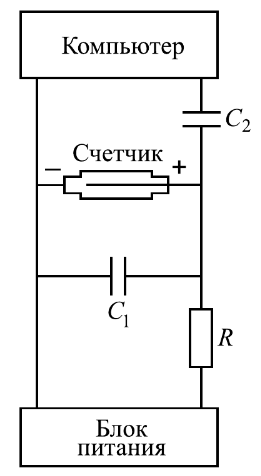
\includegraphics[scale = 0.5]{pictures/scheme.png}
		\caption{Схема включения датчика}
	\end{figure}



	\section{Используемое оборудование}

	\section{Результаты измерений и обработка данных}
	\section{Обсуждение результатов}
	\section{Вывод}
\end{document}
